\documentclass{beamer}
\mode<presentation> {
\usepackage{color}
\definecolor{bottomcolour}{rgb}{0.21,0.11,0.21}
\definecolor{middlecolour}{rgb}{0.21,0.11,0.21}
\setbeamercolor{structure}{fg=white}
\setbeamertemplate{frametitle}[default]%[center]
\setbeamercolor{normal text}{bg=black, fg=white}
\setbeamertemplate{background canvas}[vertical shading]
[bottom=bottomcolour, middle=middlecolour, top=black]
\setbeamertemplate{items}[circle]
\setbeamertemplate{navigation symbols}{} %no nav symbols
\setbeamercolor{block title}{use=structure,fg=white,bg=structure.fg!50!red!50!blue!100!green}
\setbeamercolor{block body}{parent=normal text,use=block title,bg=block title.bg!5!white!10!bg,fg=white}
\setbeamertemplate{navigation symbols}{}
}
\usepackage{graphicx} 
\usepackage{booktabs} 
\usepackage[utf8]{inputenc}  
\usepackage[T1]{fontenc}  
\usepackage{geometry}     
%\usepackage[francais]{babel} 
\usepackage{eurosym}
\usepackage{verbatim}
\usepackage{ragged2e}
\justifying

%%%%%%%%%%%%%%%%%%%%%%%%%%%%%%%%%%%%%%%%%%%%%%%%%%%%%%%%%%%%%%%%
%% ccBeamer 0.1, 2007-07-02                                   %%
%% Written by Sebastian Pipping <webmaster@hartwork.org>      %%
%% ---------------------------------------------------------- %%
%% Licensed under Creative Commons Attribution-ShareAlike 3.0 %%
%% http://creativecommons.org/licenses/by-sa/3.0/             %%
%%%%%%%%%%%%%%%%%%%%%%%%%%%%%%%%%%%%%%%%%%%%%%%%%%%%%%%%%%%%%%%%


%% Images
\newcommand{\CcImageBy}[1]{%
	
\includegraphics[scale=#1]{creative_commons/cc_by_30.pdf}%
}
\newcommand{\CcImageCc}[1]{%
	
\includegraphics[scale=#1]{creative_commons/cc_cc_30.pdf}%
}
\newcommand{\CcImageDevNations}[1]{%
	
\includegraphics[scale=#1]{creative_commons/cc_dev_nations_30.pdf}%
}
\newcommand{\CcImageNc}[1]{%
	
\includegraphics[scale=#1]{creative_commons/cc_nc_30.pdf}%
}
\newcommand{\CcImageNd}[1]{%
	
\includegraphics[scale=#1]{creative_commons/cc_nd_30.pdf}%
}
\newcommand{\CcImagePd}[1]{%
	
\includegraphics[scale=#1]{creative_commons/cc_pd_30.pdf}%
}
\newcommand{\CcImageSa}[1]{%
	
\includegraphics[scale=#1]{creative_commons/cc_sa_30.pdf}%
}
\newcommand{\CcImageSampling}[1]{%
	
\includegraphics[scale=#1]{creative_commons/cc_sampling_30.pdf}%
}
\newcommand{\CcImageSamplingPlus}[1]{%
	
\includegraphics[scale=#1]{creative_commons/cc_sampling_plus_30.pdf}%
}


%% Groups
\newcommand{\CcGroupBy}[1]{% zoom
	\CcImageBy{#1}%
}
\newcommand{\CcGroupByNc}[2]{% zoom, gap
	\CcImageBy{#1}\hspace*{#2}\CcImageNc{#1}%
}
\newcommand{\CcGroupByNcNd}[2]{% zoom, gap
	\CcImageBy{#1}\hspace*{#2}\CcImageNc{#1}\hspace*{#2}\CcImageNd{#1}%
}
\newcommand{\CcGroupByNcSa}[2]{% zoom, gap
	\CcImageBy{#1}\hspace*{#2}\CcImageNc{#1}\hspace*{#2}\CcImageSa{#1}%
}
\newcommand{\CcGroupByNd}[2]{% zoom, gap
	\CcImageBy{#1}\hspace*{#2}\CcImageNd{#1}%
}
\newcommand{\CcGroupBySa}[2]{% zoom, gap
	\CcImageBy{#1}\hspace*{#2}\CcImageSa{#1}%
}
\newcommand{\CcGroupDevNations}[1]{% zoom
	\CcImageDevNations{#1}%
}
\newcommand{\CcGroupNcSampling}[2]{% zoom, gap
	\CcImageNc{#1}\hspace*{#2}\CcImageSampling{#1}%
}
\newcommand{\CcGroupPd}[1]{% zoom
	\CcImagePd{#1}%
}
\newcommand{\CcGroupSampling}[1]{% zoom
	\CcImageSampling{#1}%
}
\newcommand{\CcGroupSamplingPlus}[1]{% zoom
	\CcImageSamplingPlus{#1}%
}


%% Text
\newcommand{\CcLongnameBy}{Attribution}
\newcommand{\CcLongnameByNc}{Attribution-NonCommercial}
\newcommand{\CcLongnameByNcNd}{Attribution-NoDerivs}
\newcommand{\CcLongnameByNcSa}{Attribution-NonCommercial-ShareAlike}
\newcommand{\CcLongnameByNd}{Attribution-NoDerivs}
\newcommand{\CcLongnameBySa}{Attribution-ShareAlike}

\newcommand{\CcNote}[1]{% longname
	This work is licensed under the \textit{Creative Commons #1 3.0 License}.%
}


\title[De l'importance de l'éducation populaire au numérique]{De l'importance de l'éducation populaire au numérique}
\author{JDLL 2016}
\author{Genma}

\begin{document}

%% Titlepage
\begin{frame}
	\titlepage
	\vfill
	\begin{center}
		\CcGroupByNcSa{0.83}{0.95ex}\\[2.5ex]
		{\tiny\CcNote{\CcLongnameByNcSa}}
		\vspace*{-2.5ex}
	\end{center}
\end{frame}

\begin{frame}
\frametitle{
\includegraphics[scale=0.4]{./images/Genma.jpg} \ \ \  A propos de moi  }
\begin{columns}[c] 
\column{.55\textwidth} 
\textbf{Où me trouver sur Internet?}
\begin{itemize}
\item Le Blog de Genma : http://genma.free.fr
\item Twitter : http://twitter.com/genma
\end{itemize}
\column{.5\textwidth} 
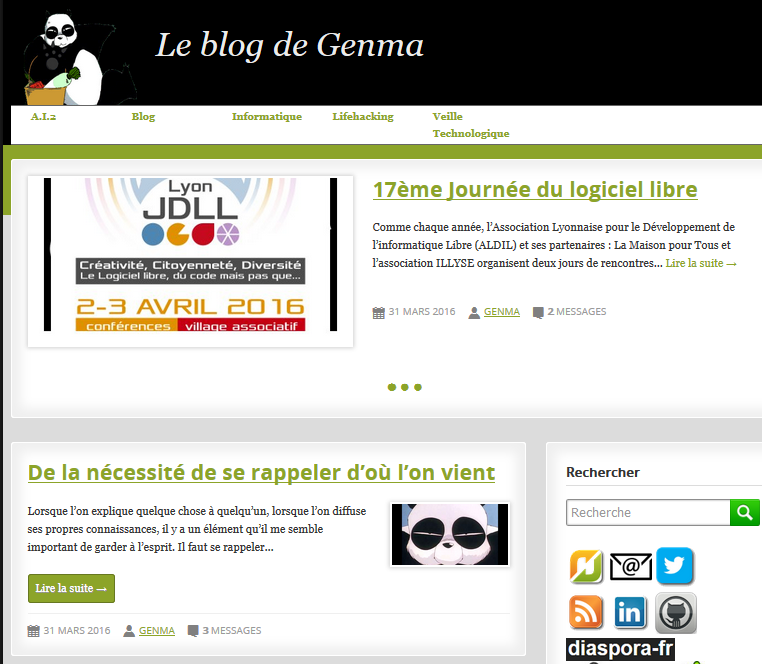
\includegraphics[scale=0.40] {./images/blog.png} 
\end{columns}
\end{frame}

%--------------------------------------------------------------------------------
\begin{frame}
\frametitle{Qui je suis?}
\begin{block}{Une expérience de \emph{vulgarisateur}}
\justifying{
\begin{itemize}
\justifying{
\item Formations, conférences et ateliers destinés au grand public, des libristes, des journalistes ou à des geeks hackitvistes...
\item Différents activités dans le milieu associatif libriste (Framasoft, FirefoxOS, Café vie privée etc.
}
\end{itemize}
}\end{block}
\end{frame}

%====================================POURQUOI=========================================
\begin{frame}
\begin{center}
\Huge {Pourquoi cette présentation?}
\end{center}
\end{frame}

%--------------------------------------------------------------------------------
\begin{frame}
\frametitle{Pourquoi cette présentation?}

\begin{block}{L’Informatique et Internet sont partout dans nos vies quotidiennes}
\justifying{
Tout à chacun soit à même de s’approprier les connaissances nécessaires et suffisantes pour comprendre ces outils qui changent les fondements mêmes de notre société, dans notre accès à l’information, aux connaissances, au partage, à la communication...}\end{block}

\begin{block}{Importance de la communication et de la vulgarisation}
\justifying{
\begin{itemize}
\item pour que l'éducation populaire se fasse ;
\item que l'on ne pense plus "RTFM" ;
\item que  chacun et chacune aura les moyens de s'approprier le numérique et de comprendre les enjeux (neutralité du net, importance de la vie privée, lutte contre les GAFAM etc.)
\end{itemize}
}\end{block}
\end{frame}

%==================================COMMENT==================================================
\begin{frame}
\begin{center}
\Huge {Comment éduquer au numérique?}
\end{center}
\end{frame}

%=================================  QUOI  ====================================
\begin{frame}
\begin{center}
\Huge {Sous quelles formes?}
\end{center}
\end{frame}

%-----------------------------------------------
\begin{frame}
\begin{center}
\Huge{Utiliser des analogies \\comme celles des recettes de cuisine...}
\end{center}
\end{frame}

%-----------------------------------------------
\begin{frame}
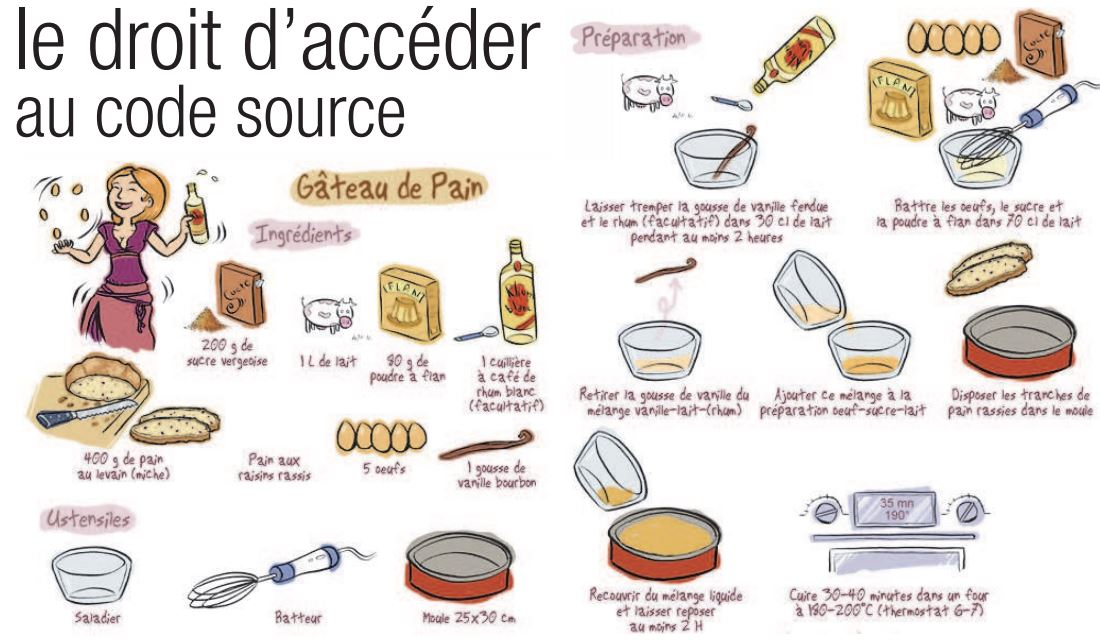
\includegraphics[scale=0.6] {./images/Cuisine01.jpg} 
\end{frame}
\begin{frame}
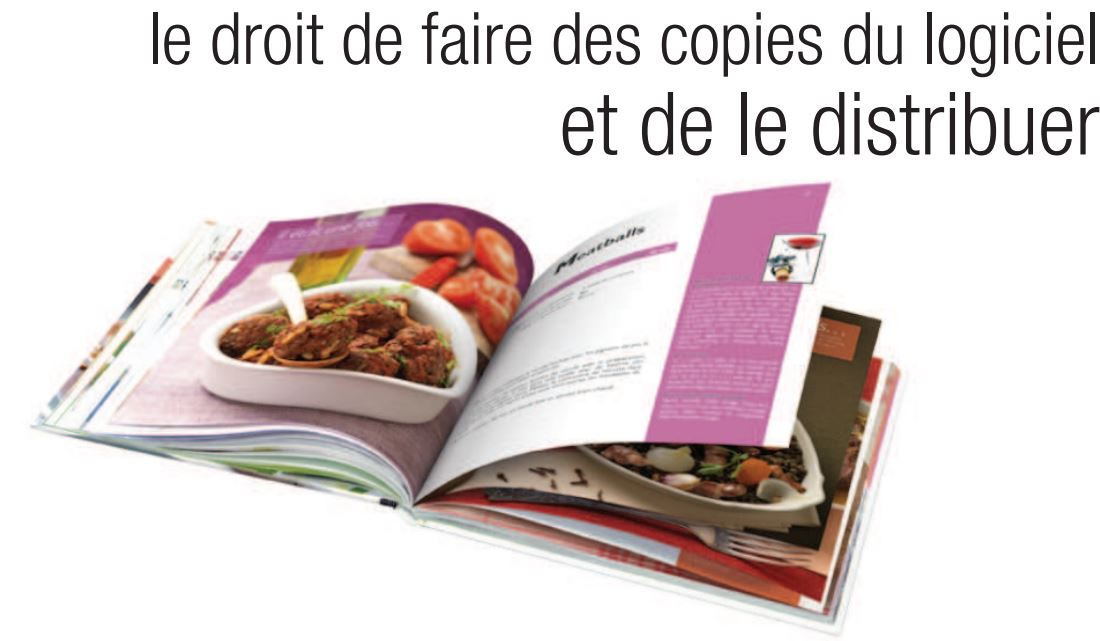
\includegraphics[scale=0.5] {./images/Cuisine02.jpg} 
\end{frame}
\begin{frame}
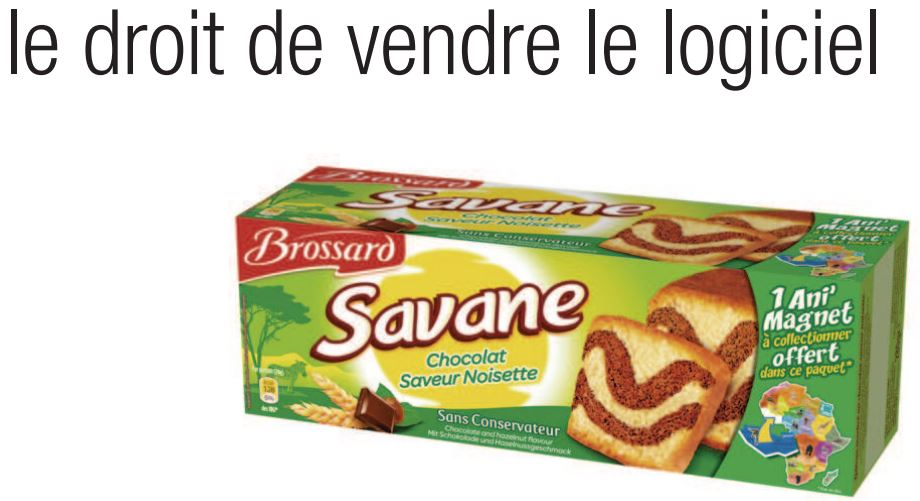
\includegraphics[scale=0.6] {./images/Cuisine03.jpg} 
\end{frame}
\begin{frame}
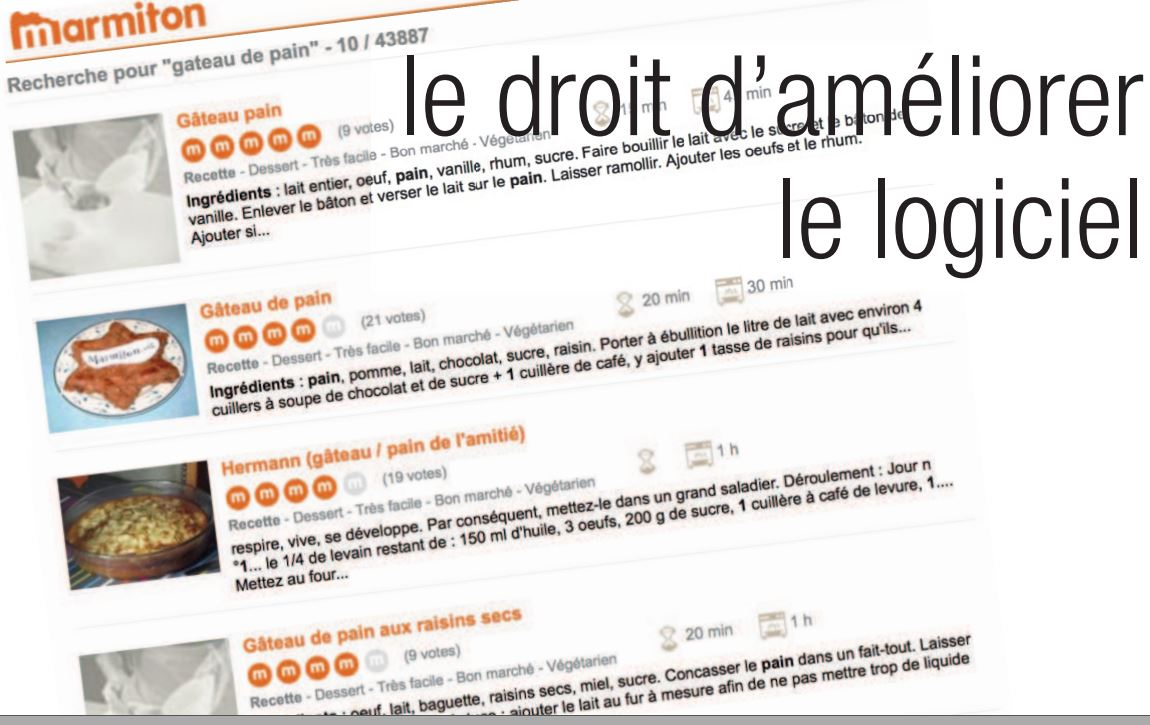
\includegraphics[scale=0.48] {./images/Cuisine04.jpg} 
\end{frame}
%-----------------------------------------------
\begin{frame}
\begin{center}
\Huge{Donner des cours d'hygiène numérique}
\\~\\
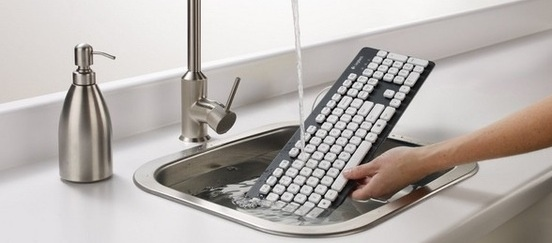
\includegraphics[scale=0.5]{./images/nettoyer_son_clavier.jpg}
\end{center}
\end{frame}

%----------------------------------------------------------------------------------------
\begin{frame}
\frametitle{L'hygiène numérique?}
\begin{block}{Une définition?}
\justifying{
L'hygiène est un ensemble de mesures destinées à prévenir les infections et l'apparition de maladies infectieuses.
\\
L'hygiène numérique, ce sont des règles destinées à mieux utiliser son ordinateur, en sécurité, de façon simple.
}
\end{block}
\end{frame}

%----------------------------------------------------------------------------------------
\begin{frame}
\frametitle{Un exemple}
\begin{block}{On me le vole mon PC}
\justifying{
\begin{itemize}
\item  Quelles sont les données que je perds? Amène la notion de \emph{sauvegarde}.
\item  Quelles sont les données que l'on trouve? Amène la notionde \emph{chiffrement}.
\end{itemize}
}
\end{block}
\begin{center}
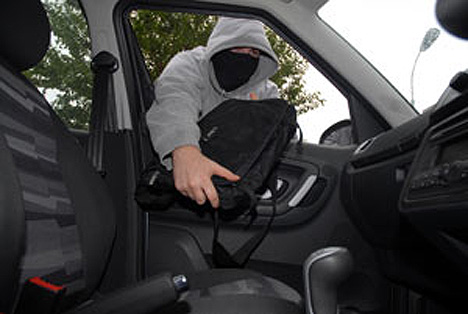
\includegraphics[scale=0.5] {./images/laptopthief.jpg}
\end{center}
\end{frame}

%-----------------------------------------------
\begin{frame}
\begin{center}
\Huge{Le monde associatif}
\end{center}
\end{frame}

%-----------------------------------------------
\begin{frame}
\frametitle{Sur Paris - Parinux}

\begin{block}{Premier Samedi du Libre (PSL)}
\justifying{Chaque premier samedi de chaque mois, les bénévoles des associations du Libre vous accueillent au Carrefour Numérique de la Cité des sciences et de l'industrie (CSI) pour une install party.\\ \url{http://premier-samedi.org/}
}
\end{block}
\begin{center}

\includegraphics[scale=0.5] {./images/parinux.png}
\end{center} 
\end{frame}
%-----------------------------------------------
\begin{frame}
\frametitle{Ubuntu Party}
\begin{block}{Ubuntu-fr}
Ubuntu Party : prochaine les 28 et 29 mai sur Paris.\\
\url{http://www.ubuntu-paris.org/}
\end{block}
\begin{center}
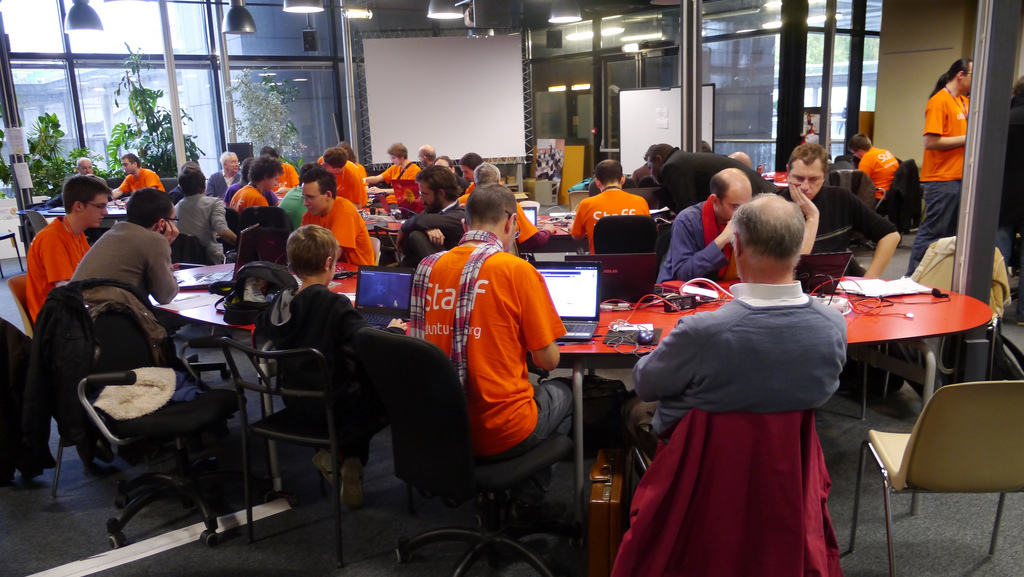
\includegraphics[scale=0.3] {./images/ubuntu-paris.jpg}
\end{center} 
\end{frame}
%-----------------------------------------------
\begin{frame}
\frametitle{Agenda du libre }
\begin{center}
\url{http://www.agendadulibre.org/}
\\
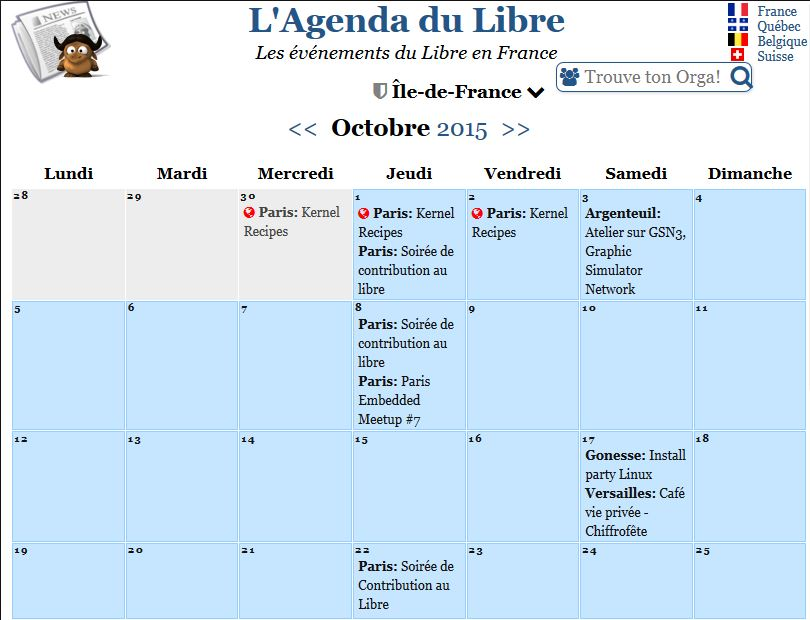
\includegraphics[scale=0.55] {./images/agenda-du-libre.jpg}
\end{center} 
\end{frame}

%----------------------------------------------------------------------------------------
\begin{frame}
\begin{center}
\Huge{Café vie privée, chiffrofête, cryptoparty}
\\~\\

\includegraphics[scale=0.3] {./images/LogoCafeViePrivee.jpg}
\end{center}
\end{frame}

%========================================================================================
\begin{frame}
\begin{center}
\Huge{Merci de votre attention}
\\
\Huge{Place aux questions.}
\\~\\

\includegraphics[scale=0.2] {./images/chat.jpg}
\end{center}
\end{frame}

%----------------------------------------------------------------------------------------
\begin{frame}
\frametitle{
\includegraphics[scale=0.4]{./images/Genma.jpg} \ \ \  Me contacter?}
\Huge{\centerline{Le Blog de Genma}}
\Huge{\centerline{http://genma.free.fr}}
\Huge{\centerline{~}}
\Huge{\centerline{Twitter : @genma}}
\end{frame}

%============================================================================================
\begin{frame}
\Huge{\centerline{ANNEXES}}
\end{frame}

%============================================================================================
\begin{frame}
\Huge{\centerline{ANNEXES}}
\end{frame}

%--------------------------------------------------------------------------------
\begin{frame}
\frametitle{Autonomie des individus parJérémie ZImmerman }
\begin{block}{Citation d'une interview donnée au podcast le Comptoir Sécu à l'occasion du FIC2016}
\justifying{
"On en a toujours parler les mains sur le clavier, les yeux sur l'écran.
Il faut parler de tout ça en des termes simples et en des termes politiques, éthiques.
Ce n'est pas y en a qu'est simple (Gmail, Mac etc.) et l'autre qui est compliqué. Non.
\\~\\Y en a qui est libre et l'autre qui est une prison.
Y en a un qui permet de comprendre, l'autre maintient dans l'ignorance
Y en a un qui permet de détenir collectivement le contrôle sur la machine, et l'autre dans lequel la machine te contrôle.
\\~\\C'est en ces termes là à mon avis qu'il faut expliquer ces choses là.
}\end{block}
\url{http://www.comptoirsecu.fr/2016/02/fic2016-2-jeremie-zimmermann-nicolas-diaz/}
\end{frame}

%----------------------------------------------------------------------------------------
\begin{frame}
\begin{center}
\frametitle{Framasoft et tous ses outils de Degooglisons}
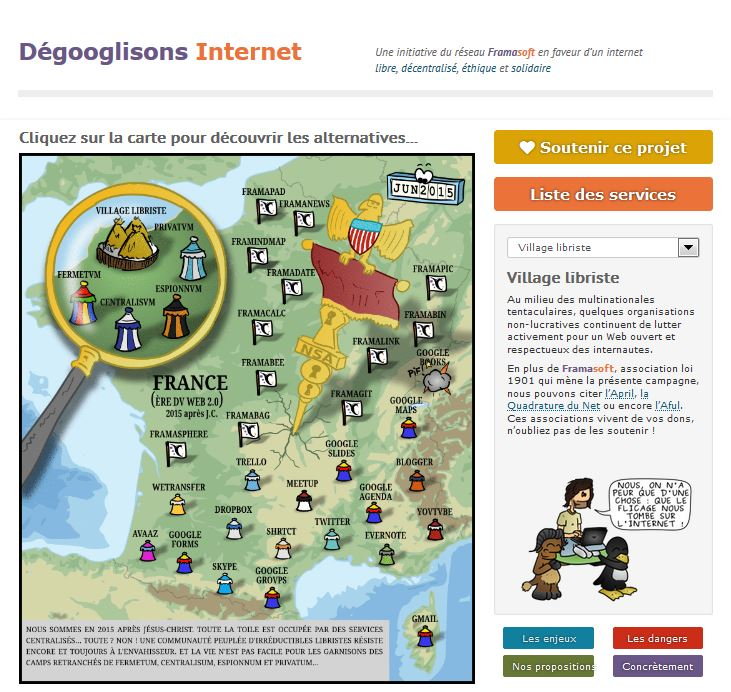
\includegraphics[scale=0.6] {./images/framasoft_degogglisons.jpg}
\end{center}
\end{frame}

%--------------------------------------------------------------------------------
\begin{frame}
\frametitle{}
\begin{block}{}
\justifying{
\begin{itemize}
\item
\item
\item
\end{itemize}
}\end{block}
\end{frame}

\end{document}